% ===============================
% Data processing
% ===============================
\newpage
\section{Data Processing}
\label{sec:dataproc}

This section targets readers who are interested in the informatics that is used to make the data available in the database, as described in the previous section. The information is of great value to everybody working with the data. Therefore, I tried to write it in a way, that every interested reader can understand the fundamentals. However, to fully understand the explanations, some knwoledge in informatics is mandatory.      

Figure \ref{fig:app_design_perl} shows an overview of the different parts involved in the data importing and analysis process. The \ac{perl} scripts which are reading data from and writing data to the database build the main part of this framework\footnote{The directories in which the scripts, modules and files are located, are listed in table \ref{tab:directories_and_files_overview} on page \pageref{tab:directories_and_files_overview}.}.

\begin{figure}[htpb]
\begin{center}
  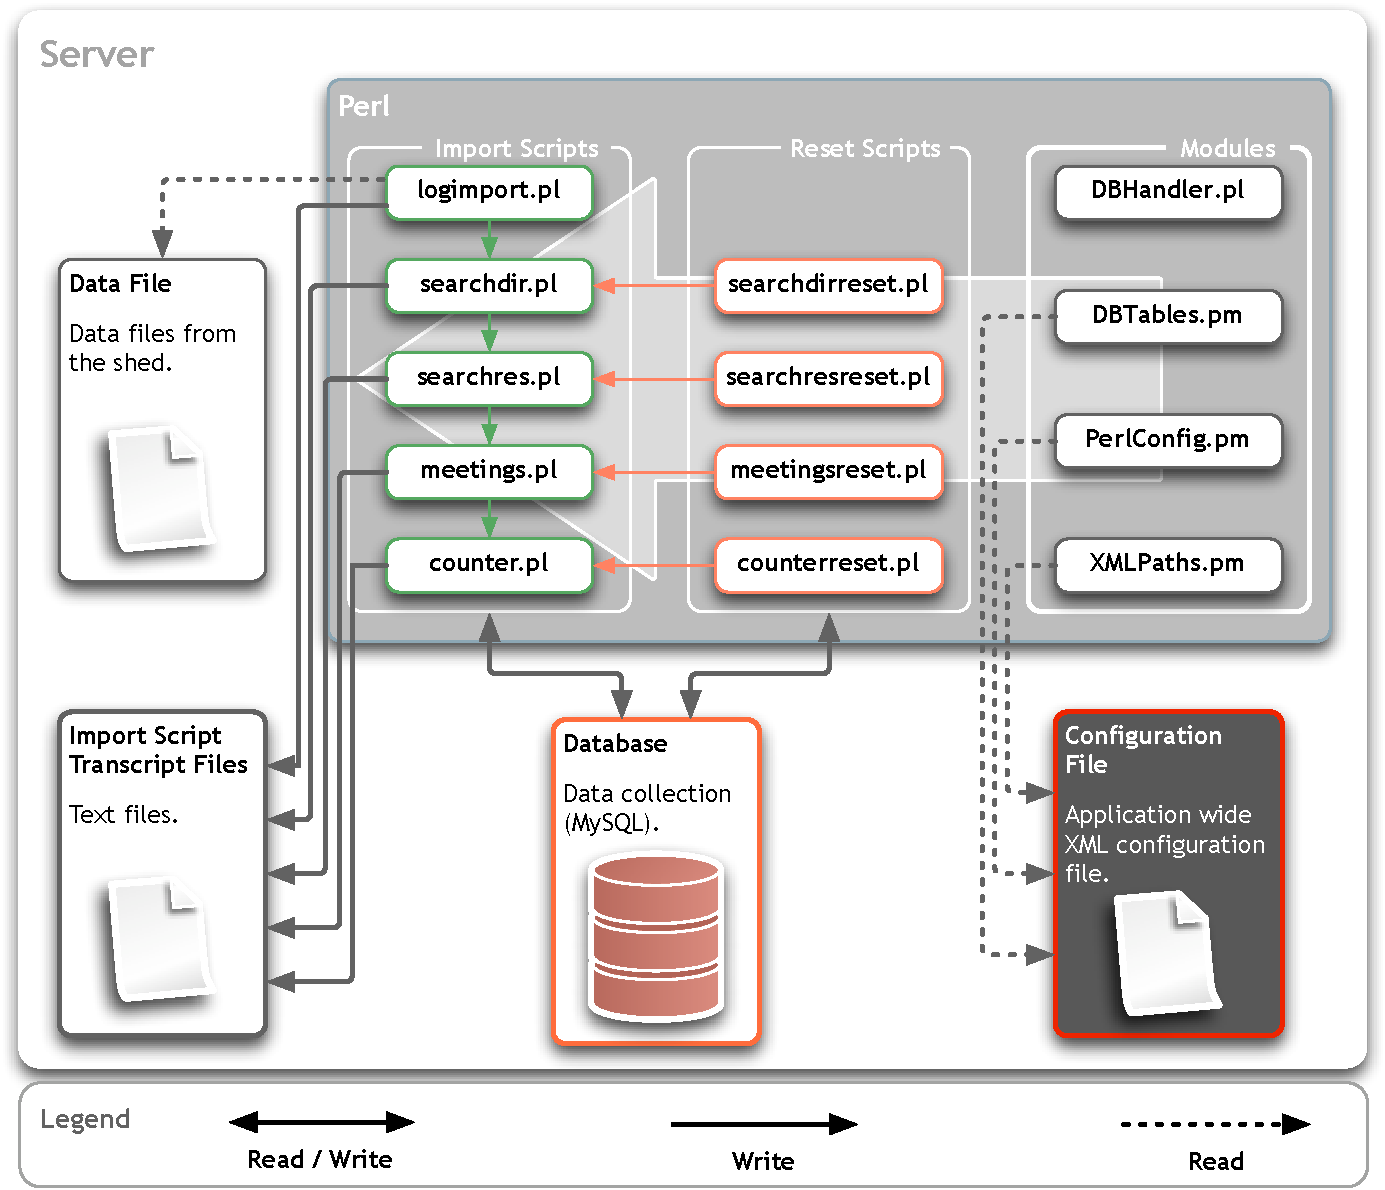
\includegraphics[width=\textwidth]{assets/pdf/app_design_perl.pdf}
  \caption[Data processing overview]{Overview of the parts involved in the data processing.}
  \label{fig:app_design_perl}
\end{center}
\end{figure}

The \textit{Import Scripts} run in a cascade, beginning with the \lstinline|logimport.pl| script, which is reading the data files from the shed, and ending with the \lstinline|counter.pl| script (indicated in figure \ref{fig:app_design_perl} by the green arrows). Each of these scrips writes a transcript file to make their progress traceable. Upon completion of the cascade, the data files are imported and stored in the respective tables as outlined in section \ref{subsec:datastorage} on page \pageref{subsec:datastorage}.

A scheduled, daily task checks for new data files uploaded to the server and starts the cascade if needed\footnote{For details about this topic see appendix \ref{app:import_schedule} on page \pageref{app:import_schedule}.}.

The \textit{Reset Scripts} set the database back to a state from where the import cascade can be rerun,  starting with the corresponding import script (indicated in figure \ref{fig:app_design_perl} by the orange arrows). If, for example, the \lstinline|searchdirreset.pl| has been executed, the import cascade can be started with the \lstinline|searchdir.pl| script\footnote{It is recommended to start the import cascade by using the import BASH scripts. This is explained in appendix \ref{app:import_schedule} on page \pageref{app:import_schedule}.}.

The \textit{Modules} read out the configuration and make it available for the import and reset scripts (indicated in figure \ref{fig:app_design_perl} by the large grey arrow with the white border). The whole configuration for the application is stored in an XML file. The part of the configuration file accountable for the perl part is shown in appendix \ref{app:configperl} on page \pageref{app:configperl}. As the perl scripts are heavily interacting with the database, the database configuration part of the configuration files is read as well by some of the \textit{Modules}\footnote{The database configuration is shown and explained in appendix \ref{app:configdb} on page \pageref{app:configdb}.}. 

The following sections provide details about each script in the import cascade.

\subsection{Importing}
\label{subsec:importing}

The \lstinline|logimport.pl| extracts the spatial position data from the data files and writes it to the \lstinline|data| table \footnote{The \lstinline|data| table structure is descriped section \ref{para:data_table} on page \pageref{para:data_table}.}.

Prior to the data extraction, the  script creates a backup of the actual database\footnote{The configuration for the backup is explained in appendix \ref{app:configperl} on page \pageref{app:configperl}.}. Subsequently the data is extracted from the data files and written to the database. 

As mentioned in section \ref{subsubsec:problems} on page \pageref{subsubsec:problems}, some of the antennas could not be addressed properly. Therefore, the script has to catch these exceptional values and convert them to the designated ones\footnote{See listing \ref{lst:antenna_adress_conversions} on page \pageref{lst:antenna_adress_conversions} for the detailed conversions.}.  

\subsection{Direction Results}
\label{subsec:dirres}

The \lstinline|searchdir.pl| script searches for matching pairs of antenna readings in the \lstinline|data| table, which build a \textit{direction result}. A pair matches if,

\begin{mylist}
\item the transponder identification values of the two readings is the same,
\item time difference in seconds between the two readings is not greater then the value set as the \lstinline|<antennaInterval>| value \footnote{See appendix \ref{app:configperl} on page \pageref{app:configperl}.} in the configuration, 
\item and the readings originate from the two different antennas attached to a box.  
\end{mylist}

Figure \ref{fig:direction_result} shows the composition of a direction \textit{in} and a direction \textit{out} result by means of an example at nestbox 16. The \lstinline|<antennaInterval>| value is set to 5 seconds.  

\begin{figure}[htpb]
\begin{center}
  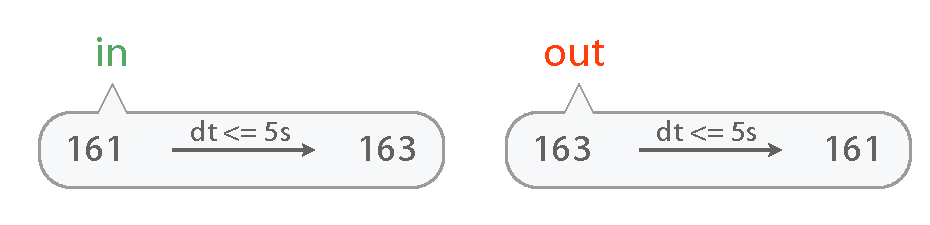
\includegraphics[width=0.75\textwidth]{assets/pdf/direction_result_schema.pdf}
  \caption[Illustration of direction result]{Illustration of the possible composition of a \textit{direction result}.}
  \label{fig:direction_result}
\end{center}
\end{figure}

This is exactly the order this script searches for \textit{direction results}. The findings are written to the \lstinline|dir| table\footnote{The \lstinline|dir| table structure described in sction \ref{para:dir_table} on page \pageref{para:dir_table}}. The value for the \lstinline|time| field of the \textit{direction result} is always taken from the antenna reading at the outer antenna. Therefore, a transpondered mouse is out of a box, when she passed the outer antenna. 

If the \lstinline|<antennaInterval>| is changed, the \lstinline| searchdirreset.pl| needs to be executed followed by the scripts in the import cascade starting with the \lstinline|searchdir.pl| script \footnotemark[14].

The \textit{direction results} are written to the \lstinline|dir| table as explaine in paragraph \ref{para:dir_table} on page \pageref{para:dir_table}. 

\subsection{Stay Results}
\label{subsec:stayres}

The \lstinline|searchres.pl| aims to find matching \textit{direction results} in the \lstinline|dir| table, which build a \textit{stay results}.

A pair matches if,

\begin{mylist}
\item the transponder identification values of the two \textit{direction results} are the same
\item the \lstinline|direction| values of the \textit{direction results} are oppositional
\item and the \textit{direction results} are recorded at the same box.
\end{mylist}

or,

\begin{mylist}
\item the transponder identification values of a \textit{direction result} with a \lstinline|direction| value of \lstinline|in| and an unused (=could not be used for a \textit{direction result}) dataset from the \lstinline|data| table recorded at an outer antenna, are the same
\item and belong to the same box.
\end{mylist}

In the former case, the \textit{stay result} is of \textbf{type 3}, in the latter case as of \textbf{type 4}. Figures \ref{fig:type_3_stay_result} and \ref{fig:type_4_stay_result} illustrate the differences between the types by means of an example of at box 16. The \lstinline|<antennaInterval>| value is set to 5 seconds. Out of the 992,128 \textit{stay results} currently in the database, 851612 (85.8\%) are type 3 results and 140516 (14.2\%) type 4 results.

\begin{figure}[htpb]
\begin{center}
  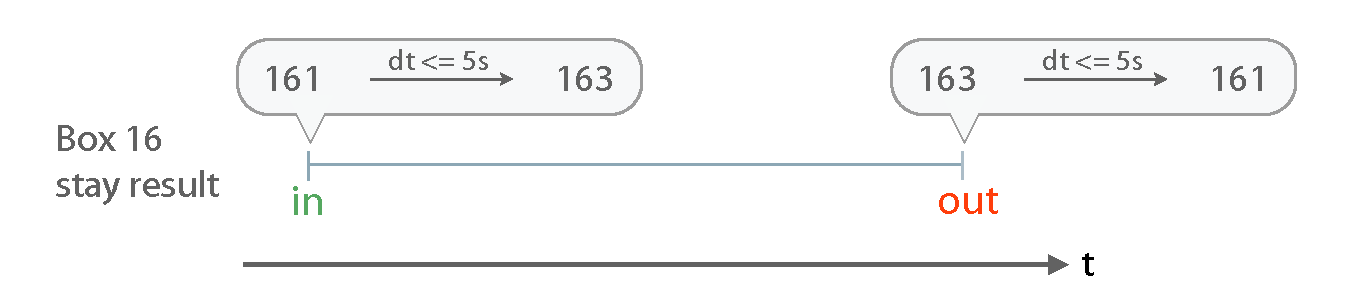
\includegraphics[width=0.75\textwidth]{assets/pdf/stay_result_type_3_schema.pdf}
  \caption[Illustration of a Type 3 \textit{stay result}]{Illustration of a Type 3 \textit{stay result} at box 16,  made up by a direction \lstinline|in| and a direction \lstinline|out| result.}
  \label{fig:type_3_stay_result}
\end{center}
\end{figure}

\begin{figure}[htpb]
\begin{center}
  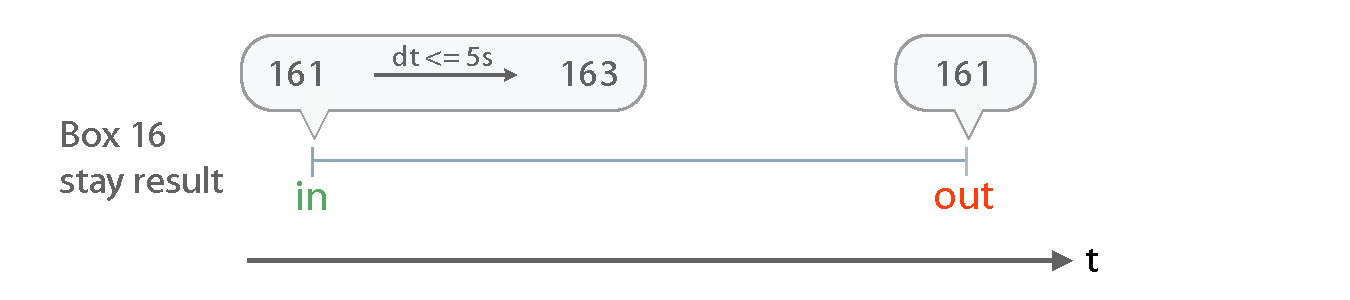
\includegraphics[width=0.75\textwidth]{assets/pdf/stay_result_type_4_schema.pdf}
  \caption[Illustration of a Type 4 \textit{stay result}]{Illustration of a Type 4 \textit{stay result} made up by a direction \lstinline|in| result and a reading at the outer antenna.}
  \label{fig:type_4_stay_result}
\end{center}
\end{figure}

Additionaly, the script has to handle the temporal overlaps of stay results. Since, the antenna system is not working perfect (see section \ref{subsubsec:problems}), if we let the script keep all possible \textit{stay results}, we get situations as illustrated in figures \ref{fig:result_overlap} and \ref{fig:result_overlap_single}. All the \textit{stay results} (1, 2 and 3) originate from the same transponder recorded at the same or different boxes. Hence, the antenna system must have missed readings, but we have no clue about the exact moment.  

In figure \ref{fig:result_overlap} we have the situation, that one \textit{stay result} (1) overlaps two others (2),(3). A reasonable explanation would be, that the antenna system missed a recordings between the \textit{in} moments of \textit{stay results} (1) and between the \textit{out} moments of \textit{stay results} (3) and (1). Since we have two \textit{stay results}, (2) and (3), which are looking valid, we discard \textit{stay result} (1), where we don't know what really happened. Furthermore, this approach is reasonable, as the probability of some, maximum two, missed antenna readings is much higher than the probabilty that eight antenna readings building two perfect looking \textit{stay results} are wrong.
 
\begin{figure}[htpb]
\begin{center}
  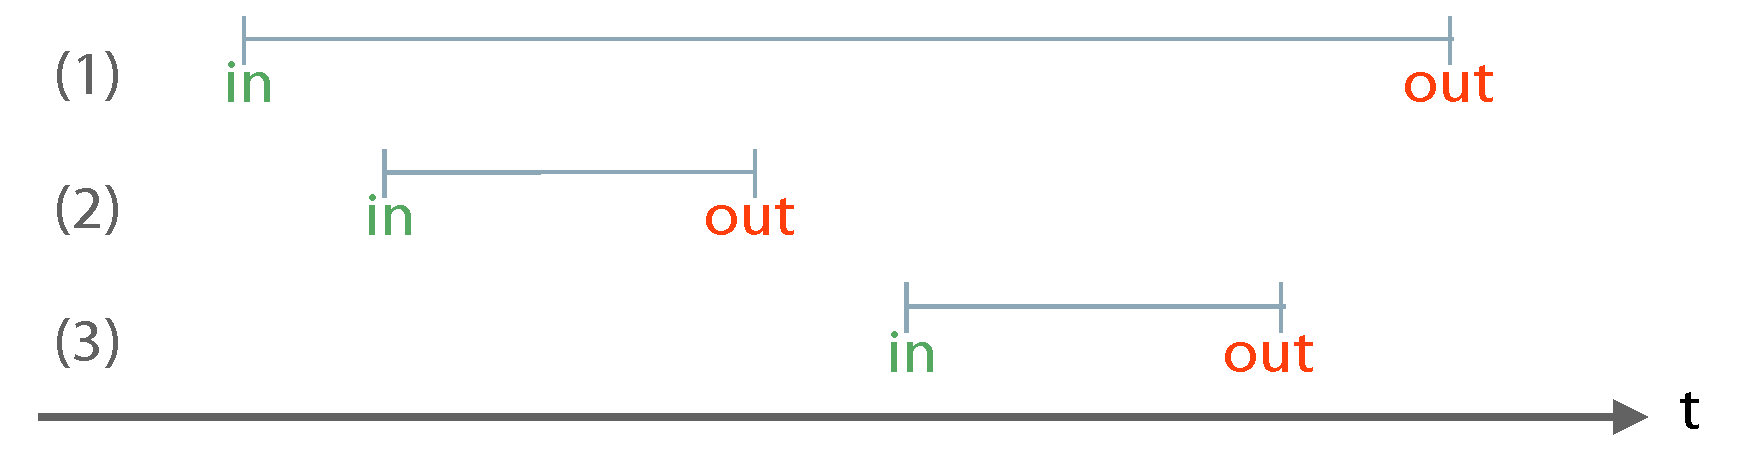
\includegraphics[width=0.75\textwidth]{assets/pdf/result_overlaps_schema.pdf}
  \caption[Multiple result overlap illustration]{Illustration of a possible result overlap situation, where a \textit{stay result} overlaps many others.}
  \label{fig:result_overlap}
\end{center}
\end{figure}

Figures \ref{fig:result_overlap_single} and \ref{fig:result_overlap_single_shifted} illustrate the situation where one \textit{stay result} overlaps another. In this case, the \textit{stay result} (1) is discarded as well.

The justification for this approach is pretty similar to the one just discussed. \textit{Stay result} (2) looks valid, but there must be missed antenna readings between the time of \textit{stay result} (1) and \textit{stay result} (2) \textit{in}, and between \textit{stay result} (2) and \textit{stay result} (1) respectively. In figure \ref{fig:result_overlap_single_shifted} the two \textit{stay results} are only partly overlapping. \textit{Stay result} (1) is discarded as well, but \textit{stay result} (2) will be discared in the next step.      

\begin{figure}[htpb]
\begin{center}
  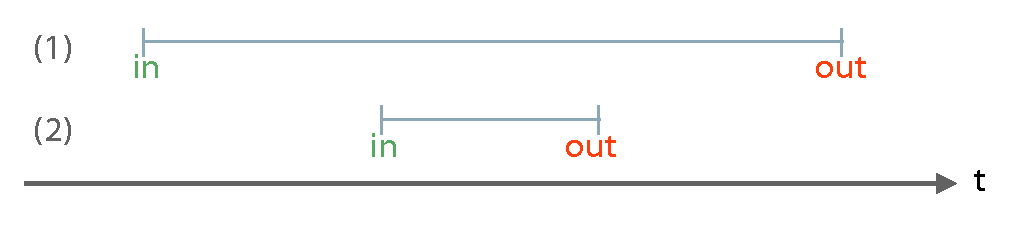
\includegraphics[width=0.75\textwidth]{assets/pdf/result_overlaps_single_schema.pdf}
  \caption[Single result fully overlap illustration]{Illustration of a possible result overlap situation, where a \textit{stay result} fully overlaps another.}
  \label{fig:result_overlap_single}
\end{center}
\end{figure} 

\begin{figure}[htpb]
\begin{center}
  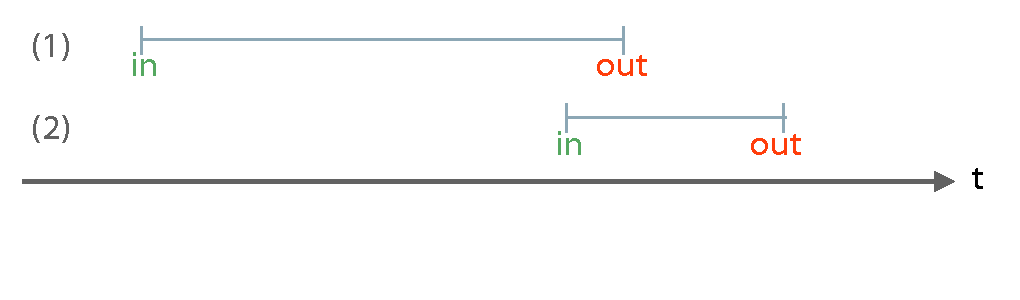
\includegraphics[width=0.75\textwidth]{assets/pdf/result_overlaps_single_shifted_schema.pdf}
  \caption[Single result partly overlap illustration]{Illustration of a possible result overlap situation, where a \textit{stay result} partly overlaps another.}
  \label{fig:result_overlap_single_shifted}
\end{center}
\end{figure}

Now, that the \textit{stay result} is checked for overlaps with other \textit{stay results}, the script checks for other antenna readings that were recorded during the \textit{stay result} as illustrated by an example in figure \ref{fig:dataset_overlap}. Obviously, only antenna readings originating from the same transponder are taken into account.

In figure \ref{fig:dataset_overlap}, four other antenna readings could be found, two of them not even from the same box. This \textit{stay result} will be discarded, as we don't know what really happened.

\begin{figure}[htpb]
\begin{center}
  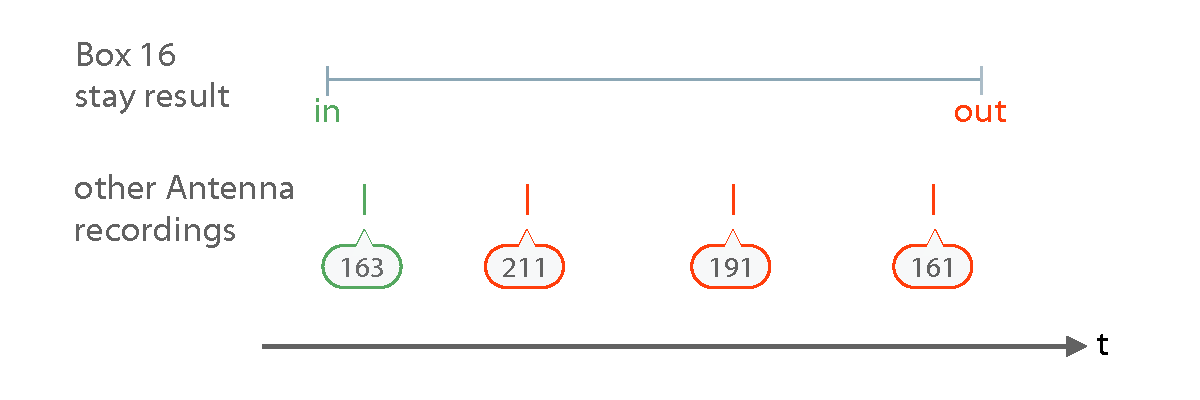
\includegraphics[width=0.75\textwidth]{assets/pdf/dataset_overlap_schema.pdf}
  \caption[Dataset overlap illustration]{Illustration of a possible dataset overlap situation, where other antenna readings have been found during a\textit{stay result}.}
  \label{fig:dataset_overlap}
\end{center}
\end{figure}

As seen in figure \ref{fig:dataset_overlap}, the reading at antenna \lstinline|163|, which is the inner antenna attached to nestbox 16, is colored green. If we have a look at the situation illustrated in figure \ref{fig:dataset_overlap_nervous}, we can see that several datasets which are exclusively recorded at the innner antenna are overlapped. In such a case, we keep the result, as the transpondered mouse has not left the box\footnote{As stated in section \ref{subsec:dirres}, a mouse is out of the box if she is recorded at the outer antenna.}, and denote it a \textit{nervous mouse}, as we think, that she is only checking the entry tube out of nervousness.

The \textit{nervous index} is simply the number of readings at the inner antenna during the \textit{stay result}, which is 4 for the situation shown in figure \ref{fig:dataset_overlap_nervous}. This value is written to the database as explained in section \ref{para:res_table}.

\begin{figure}[htpb]
\begin{center}
  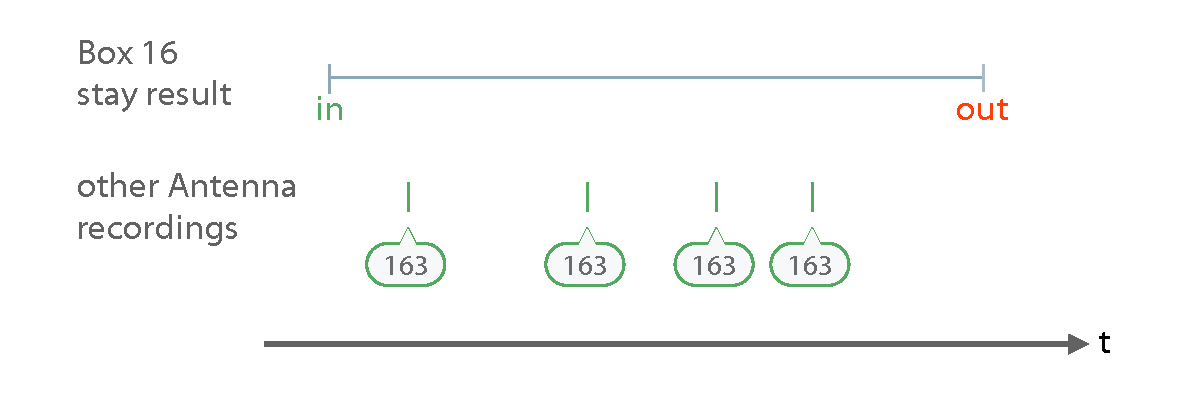
\includegraphics[width=0.75\textwidth]{assets/pdf/dataset_overlap_nervous_schema.pdf}
  \caption[Dataset overlap illustration]{Illustration of a possible dataset overlap situation, where other antenna readings have been found during a \textit{stay result}, but only at the inner antenna of the box. Such a situation is termed a \textit{nervous mouse}.}
  \label{fig:dataset_overlap_nervous}
\end{center}
\end{figure}

The searches for the \textit{stay result} overlaps and the overlapped antenna recordings could be combined. Though, we are interested in the influence of these steps on the numbers. In the period from the 5 of April 2007 to the 27 of March 2009, 1,499,110 \textit{direction results} with a direction value of \lstinline|in| are found. Without any overlap filtering, the script finds a \textit{stay result} for 1,484,458 (99.0\%) . After excluding the \textit{stay result} overlaps, 1,020,983 (68.1\%) remain, and 992,128 (66.2\%) after excluding the \textit{stay results} with overlapping antenna readings. Though, 591,549 (59.6\%) of the remaining \textit{stay results} are \textit{nervous mouse} results.

Nevertheless, an incosistancy remains. 536 (0.05\%) of the \textit{stay result} show a duration of stay longer than nine hours. Biologically these values are impractical, as, for instance, the mice have to drink outside of the nestbox. However, these results exist in the database and have been validated. A number of explanations have been discussed how such results can arise, which are quite comlicated and unlikely, but therefore could be true for these exceptional cases. These results can be excluded to be shown in the user interface (see section \ref{subsec:miceminer_config} on page \pageref{subsec:miceminer_config}), but remain in the database.     

The \textit{stay results} are written to the \lstinline|res| table as described in paragraph \ref{para:res_table} on page \pageref{para:res_table}.

\subsection{Meeting Results}
\label{subsec:meetingres}

The \lstinline|meetings.pl| script determines, when and how many time the transpondered mice spend together in the nestboxes. The \textit{stay results} make the basis. A \textit{meeting result} is found, whenever

\begin{mylist}
\item two \textit{stay results},
\item of two different transpondered mice,
\item which take place in the same nestbox,
\item temporally overlap.
\end{mylist}

Additionaly, the script analyses, how the mice meet. There are four different possibilities, as shown in figure \ref{fig:meeting_types} and explained in the follwing list.

\begin{mydesc}
\label{list:meeting_types}
\item \textbf{Type 1}: Tr. B entered the nestbox, while Tr. A was already in the box, and Tr. B left the nestbox, while Tr. A was still in the box. 
\item \textbf{Type 2}: Tr. A entered the nestbox, while Tr. B was already in the box, and Tr. A left the nestbox, while Tr. B was still in the box. 
\item \textbf{Type 3}: Tr. A entered the nestbox, while Tr. B was already in the box, and Tr. B left the nestbox, while Tr. A was still in the box. 
\item \textbf{Type 4}: Tr. A entered the nestbox, while Tr. B was already in the box, and Tr. B left the nestbox, while Tr. A was still in the box. 
\end{mydesc}

\begin{figure}[htpb]
\begin{center}
  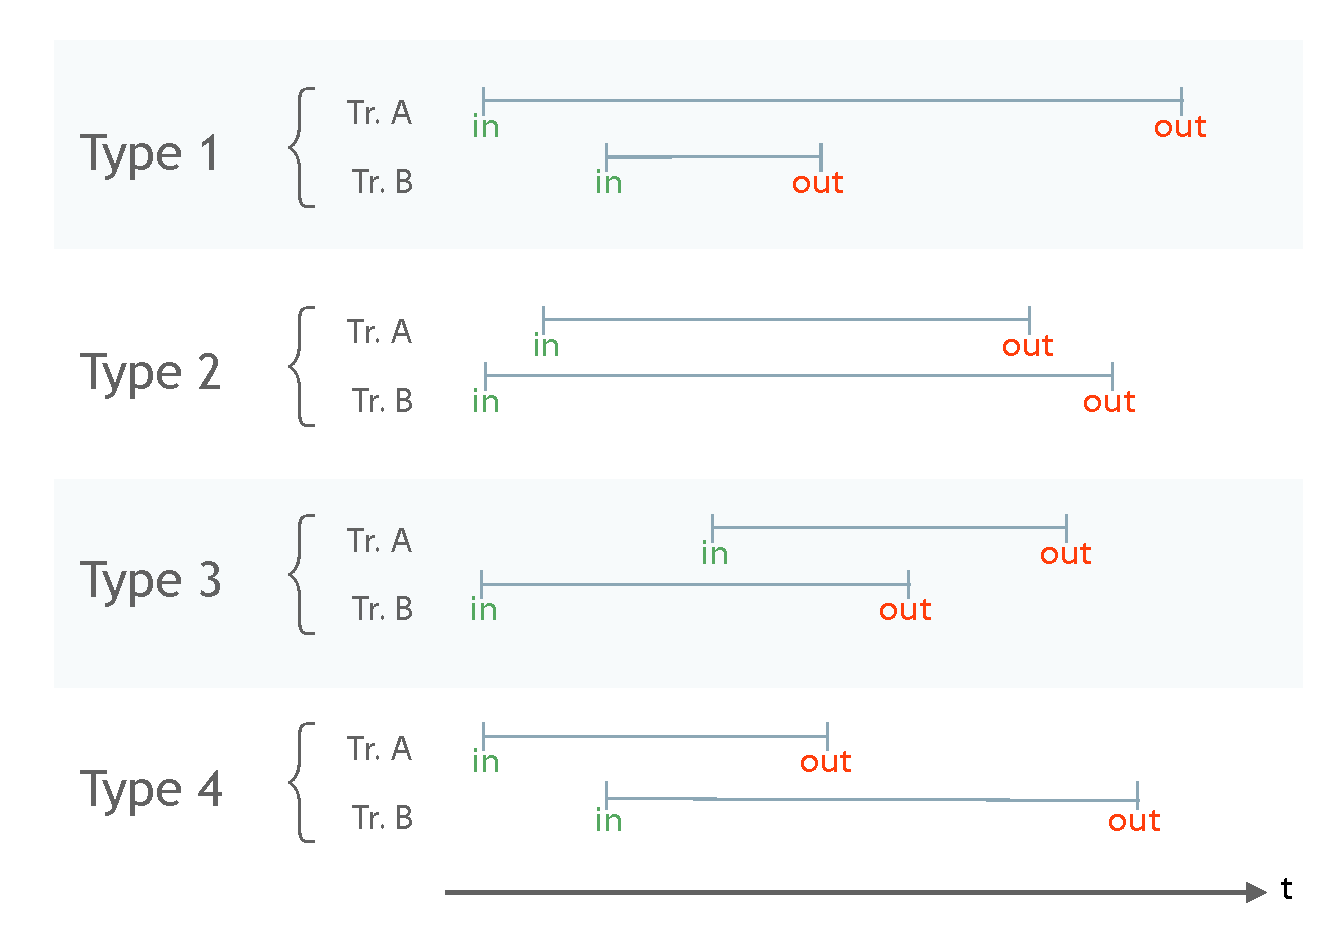
\includegraphics[width=0.75\textwidth]{assets/pdf/meeting_types_schema.pdf}
  \caption[Meeting resulst types illusttration]{Illustration of the possible meeting situations in a nestbox between two transpondered mice (Tr. A , Tr. B).}
  \label{fig:meeting_types}
\end{center}
\end{figure}

However, the \textit{meeting result} types and explanations above, only apply, if we look at the situations from the point of view of transpondered mice Tr. A. When looking at the situations from Tr. B, the types are swappaed as follows\footnote{When using the \textit{miceminer Graph Data} interface to retrieve the data, these adjustments are already done (see \ref{sec:netexp})}.

\begin{mylist}
\item Type 1 is swapped to \textbf{Type 2}   
\item Type 2 is swapped to \textbf{Type 1}
\item Type 3 is swapped to \textbf{Type 4} 
\item Type 4 is swapped to \textbf{Type 3}
\end{mylist}

As already mentioned in the section about the \textit{stay results}, a few exceptional results show an impossible duration of stay. Since the \textit{meeting results} are derived from the \textit{stay results}, there exist some impossible \textit{meeting results} (97 or 0.01\%).  

The \textit{meeting results}, including the \textit{type} values are written to the \lstinline|meetings| table as described in paragraph \ref{para:meetings_table} on page \pageref{para:meetings_table}. These results can be excluded to be displayed in the user interface as well by setting the \lstinline|<maxStay>| value in the configuration, as explained in section \ref{subsec:miceminer_config} on page \pageref{subsec:miceminer_config}, but remain in the database.
